\documentclass[11pt]{article}

\usepackage[letterpaper,margin=1in]{geometry}
\usepackage[T1]{fontenc}
\usepackage[utf8]{inputenc}
\usepackage{booktabs}
\usepackage{array}
\usepackage{enumitem}
\usepackage{xcolor}
\usepackage{listings}
\usepackage{tikz}
\usetikzlibrary{arrows.meta,positioning}
\usepackage[hidelinks]{hyperref}

\definecolor{codebg}{RGB}{247,249,250}
\definecolor{codeframe}{RGB}{220,224,228}
\definecolor{accent}{RGB}{27,94,72}

\lstset{
  basicstyle=\ttfamily\small,
  backgroundcolor=\color{codebg},
  frame=single,
  rulecolor=\color{codeframe},
  breaklines=true,
  showstringspaces=false,
  columns=fullflexible,
  keepspaces=true,
  aboveskip=1em,
  belowskip=1em
}

\title{
  \vspace{-2em}
  \textbf{ResonantOS SDK Reference Demo}\\[0.4em]
  \large Technical Report and User Guide
}

\author{ResonantOS SDK Working Group}
\date{September 24, 2026}

\begin{document}

\maketitle

\begin{abstract}
This report documents the ResonantOS SDK reference demonstration
(\textsc{SDK-DEMO-002}), in which three independently packaged add-ons are
discovered, validated, opened, and exercised inside the real ResonantOS browser
extension through a single generic contract, with no add-on-specific code in
ResonantOS Core. It describes the objectives, the architecture that was
verified, the reference add-ons that were built, the capability and isolation
model, the engineering problems that were found and corrected, the test
results, and a step-by-step user guide for reproducing the demonstration.
\end{abstract}

\tableofcontents

\section{Objectives}

The goal of this work was to move the ResonantOS SDK from an architectural
proposal to a working, browser-visible demonstration. Specifically, the
demonstration had to answer one question:

\begin{quote}
\itshape
Can a developer create a new, interactive ResonantOS add-on through a generic
SDK contract, have ResonantOS discover it, expose its declared capabilities and
trust boundary, open it inside the real browser extension, communicate with it,
and disable or remove it --- all without adding add-on-specific logic to
ResonantOS Core?
\end{quote}

The acceptance criteria were intentionally strict. The demonstration had to
run in the actual ResonantOS Chrome extension (not a mock page and not a
terminal trace), and it had to prove the following properties:

\begin{itemize}[leftmargin=1.5em]
  \item \textbf{Generic discovery} --- an independently packaged add-on is
        discovered without teaching Core its identifier.
  \item \textbf{Manifest-driven contract} --- identity, version, capabilities,
        permissions, and contributions come from the add-on's own manifest.
  \item \textbf{Isolation} --- add-on UI runs in a sandboxed, cross-origin
        context and cannot reach ResonantOS internals.
  \item \textbf{Capability enforcement} --- an allowed operation succeeds; an
        unauthorized operation is refused at the boundary.
  \item \textbf{Replacement proof} --- at least two unrelated add-ons register
        through the same mechanism, and a third, tutorial-style add-on teaches
        the SDK while itself running through that mechanism.
\end{itemize}

\section{Architecture Overview}

The SDK is a \emph{plug/socket} contract, not a replacement for ResonantOS
architecture. On one side is the trusted ResonantOS Core; on the other is the
replaceable add-on world; between them is the SDK boundary through which every
interaction must travel.

\begin{center}
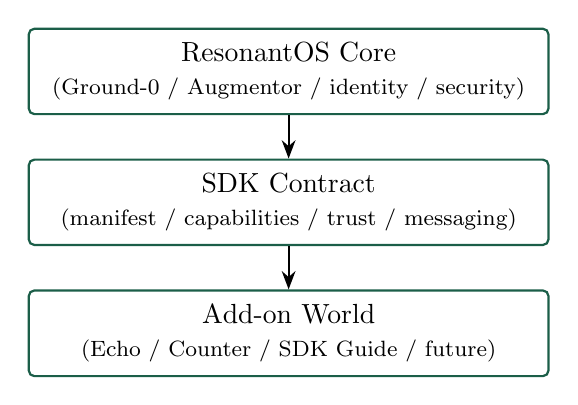
\begin{tikzpicture}[
  node distance=0.55cm,
  box/.style={draw=accent, thick, rounded corners=2pt, align=center,
              inner sep=5pt, minimum width=6.6cm},
  arrow/.style={-{Stealth}, thick}
]
  \node[box] (core) {ResonantOS Core \\ \footnotesize(Ground-0 / Augmentor / identity / security)};
  \node[box, below=of core] (sdk) {SDK Contract \\ \footnotesize(manifest / capabilities / trust / messaging)};
  \node[box, below=of sdk] (addons) {Add-on World \\ \footnotesize(Echo / Counter / SDK Guide / future)};
  \draw[arrow] (core) -- (sdk);
  \draw[arrow] (sdk) -- (addons);
\end{tikzpicture}
\end{center}

The end-to-end pipeline that a workspace add-on traverses is:

\begin{center}
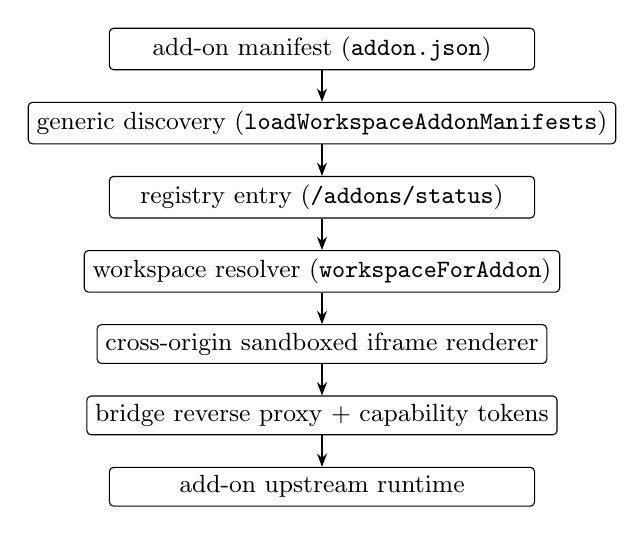
\begin{tikzpicture}[
  node distance=0.4cm,
  stage/.style={draw, rounded corners=1.5pt, align=center, inner sep=3pt,
                minimum width=5.4cm, font=\small},
  arrow/.style={-{Stealth}}
]
  \node[stage] (m) {add-on manifest (\texttt{addon.json})};
  \node[stage, below=of m] (d) {generic discovery (\texttt{loadWorkspaceAddonManifests})};
  \node[stage, below=of d] (r) {registry entry (\texttt{/addons/status})};
  \node[stage, below=of r] (w) {workspace resolver (\texttt{workspaceForAddon})};
  \node[stage, below=of w] (i) {cross-origin sandboxed iframe renderer};
  \node[stage, below=of i] (b) {bridge reverse proxy + capability tokens};
  \node[stage, below=of b] (u) {add-on upstream runtime};
  \draw[arrow] (m) -- (d);
  \draw[arrow] (d) -- (r);
  \draw[arrow] (r) -- (w);
  \draw[arrow] (w) -- (i);
  \draw[arrow] (i) -- (b);
  \draw[arrow] (b) -- (u);
\end{tikzpicture}
\end{center}

\subsection{Isolation and token delivery}

The key security decision is how add-on code executes. Add-ons render inside a
sandboxed \texttt{iframe} whose \texttt{src} is the add-on's own upstream
origin (for example \url{http://127.0.0.1:47321}), using the sandbox
\texttt{allow-scripts} plus \texttt{allow-same-origin}. Because the iframe is
same-origin with its own upstream and cross-origin from the extension, it can
fetch its own API without CORS, yet cannot reach the extension's
\texttt{chrome.*} APIs, extension storage, or the bridge.

Capability tokens are delivered from the trusted extension to the add-on iframe
via \texttt{postMessage} (with \texttt{targetOrigin} set to the add-on's own
origin). The add-on validates the message before trusting it. The bridge token
is \emph{never} delivered to the add-on, and no \texttt{Access-Control-Allow-Origin}
header is used in the add-on upstreams.

\section{The Reference Add-ons}

Three add-ons were built, all registered through the same generic mechanism
with zero Core changes:

\begin{center}
\begin{tabular}{@{}p{3.1cm}p{3.0cm}p{3.2cm}p{3.6cm}@{}}
\toprule
\textbf{Add-on} & \textbf{ID} & \textbf{Upstream port} & \textbf{Purpose} \\
\midrule
Resonant Echo & \texttt{addon.resonant-echo} & 47321 & Deterministic echo; proves the message round-trip \\
Resonant Counter & \texttt{addon.resonant-counter} & 47422 & Second add-on; proves the mechanism is generic \\
SDK Guide & \texttt{addon.sdk-guide} & 47423 & Interactive tutorial; teaches the SDK while using it \\
\bottomrule
\end{tabular}
\end{center}

\subsection{Resonant Echo}

A deterministic echo responder. A user types a message and the add-on returns
\texttt{Resonant Echo received: "<message>"}. It has no model, no provider, and
no network dependency. Its routes are \texttt{GET /api/echo/status} and
\texttt{POST /api/echo/message}, both gated on the \texttt{harness-messaging}
capability.

\subsection{Resonant Counter}

A deterministic counter. It exposes \texttt{POST /api/counter/increment} and
\texttt{GET /api/counter/read}. Its existence is the \emph{replacement proof}:
a second, unrelated add-on onboards through the exact same mechanism with no
additional Core code.

\subsection{SDK Guide}

A tutorial add-on that walks any user through what the SDK is, how an add-on is
discovered and activated, what it can and cannot do, and what has been built.
Its interactive steps perform \emph{real} bridge-mediated calls: a live message
round-trip and a deliberately denied action that returns \texttt{403}. This is
the strongest form of the replacement proof --- an add-on that teaches the SDK
while itself being an SDK add-on.

\section{Capability and Security Model}

Each add-on declares its capabilities in its manifest. The capability boundary
is enforced at the bridge \emph{and} re-checked at the add-on's own upstream.

\begin{center}
\begin{tabular}{@{}p{3.4cm}p{7.6cm}@{}}
\toprule
\textbf{Status} & \textbf{Capabilities} \\
\midrule
Granted & \texttt{harness-messaging} (the single capability the reference
           add-ons use to send and receive messages) \\
\hline
Denied & \texttt{wallet-signing}, \texttt{provider-secret-read},
         \texttt{trusted-memory-write}, \texttt{filesystem-write} \\
\bottomrule
\end{tabular}
\end{center}

The security posture that was verified:

\begin{itemize}[leftmargin=1.5em]
  \item The add-on iframe is isolated (cross-origin sandbox) and cannot reach
        extension storage, \texttt{chrome.*} APIs, or the bridge.
  \item Capability tokens are minted by the extension via the bridge and
        delivered to the iframe over \texttt{postMessage}; they are never
        placed in served HTML or a URL.
  \item The bridge token never reaches the add-on.
  \item No \texttt{Access-Control-Allow-Origin} header is emitted by the add-on
        upstreams.
  \item Unauthorized requests fail closed with \texttt{403}.
\end{itemize}

\section{How It Was Built}

\subsection{Engineering problems found and corrected}

The independent review loop surfaced and fixed a series of real defects that
the initial automated suite did not catch. These are recorded because they
explain \emph{why} the demonstration now works, and why a browser-visible test
is a necessary gate:

\begin{enumerate}[leftmargin=1.5em]
  \item \textbf{SyntaxError in the workspace module} --- an \texttt{await}
        inside a non-\texttt{async} function broke the workspace page; the
        module was made \texttt{async} and a syntax gate was added to catch
        this class of error in CI.
  \item \textbf{Inline script dropped by CSP} --- the extension's
        \texttt{script-src} policy silently dropped inline scripts in
        \texttt{srcdoc} iframes, leaving the add-on UI dead.
  \item \textbf{Missing token delivery} --- the bootstrap endpoint was
        capability-gated while nothing actually delivered the capability token
        to the iframe (a chicken-and-egg).
  \item \textbf{Insecure CORS workaround} --- an
        \texttt{Access-Control-Allow-Origin: null} plus HTML-templated tokens
        created a cross-origin read channel; this was replaced with
        \texttt{postMessage} delivery.
  \item \textbf{Port not surfaced} --- the registry entry derived the upstream
        port from an environment variable rather than the manifest's
        \texttt{runtime.port}, so the renderer fell back to a non-isolated path
        and never delivered the bootstrap.
  \item \textbf{Collapsed iframe} --- the add-on iframe had no height
        propagation and rendered at the browser's 150\,px default, clipping the
        input and Send button.
\end{enumerate}

\subsection{Test hardening}

A dedicated unit test now pins the port-derivation logic
(\texttt{buildWorkspaceAddonRegistryEntry}) so a regression of the
\texttt{runtime.port} mapping is caught automatically. The real-extension
browser test was changed to route its mock \texttt{/addons/status} response
through the production derivation rather than hard-coding the port.

\section{Test Results}

\begin{center}
\begin{tabular}{@{}p{8.6cm}p{4.6cm}@{}}
\toprule
\textbf{Suite} & \textbf{Result} \\
\midrule
\texttt{npm run build} & PASS \\
\texttt{npm run test:extension-syntax} & 2/2 PASS \\
\texttt{npm run test:browser-host} & 13/13 PASS \\
\texttt{npm run test:browser-first} & 1298 PASS / 0 FAIL / 1 env-skip \\
\texttt{npm test} (Vitest) & 487/487 PASS \\
\bottomrule
\end{tabular}
\end{center}

The single skip is environment-dependent: an in-process intake test skips when
another bridge instance is already holding the add-on ports. On a clean machine
the run is \texttt{0 skip}. The real-extension browser tests additionally
verify the visible click-through (Echo send, Counter increment, SDK Guide live
message and denied action, and the unauthorized \texttt{403}).

\section{User Guide}

This section describes how to reproduce the demonstration from a clean checkout.

\subsection{Prerequisites}

\begin{itemize}[leftmargin=1.5em]
  \item Node.js \texttt{>= 22.13.0} (see \texttt{.nvmrc}).
  \item Google Chrome (for loading the unpacked extension).
\end{itemize}

\subsection{Checkout and install}

\begin{lstlisting}[language=bash]
git clone https://github.com/vonstegen/2.0.0-alpha.git
cd 2.0.0-alpha
git checkout r-and-d/sdk-demo-002-cross-origin-addons
npm install
\end{lstlisting}

\subsection{Place the add-ons where the bridge discovers them}

The bridge reads workspace add-ons from the user root
(\texttt{\textasciitilde/ResonantOS\_User/BrowserFirst/addons}), not from the
repository. Copy (do not symlink) the three add-on directories:

\begin{lstlisting}[language=bash]
mkdir -p ~/ResonantOS_User/BrowserFirst/addons
cp -R browser-first/addons/resonant-echo   ~/ResonantOS_User/BrowserFirst/addons/
cp -R browser-first/addons/resonant-counter ~/ResonantOS_User/BrowserFirst/addons/
cp -R browser-first/addons/sdk-guide        ~/ResonantOS_User/BrowserFirst/addons/
\end{lstlisting}

\subsection{Start the bridge}

\begin{lstlisting}[language=bash]
node run-bridge-minimal.mjs --bridge-port=47773
\end{lstlisting}

Leave the bridge running. It spawns the three add-on upstreams and writes the
generated bridge configuration that the extension reads.

\subsection{Load the extension}

\begin{enumerate}[leftmargin=1.5em]
  \item In Chrome, open \texttt{chrome://extensions}.
  \item Enable \textbf{Developer mode}.
  \item Choose \textbf{Load unpacked} and select
        \texttt{browser-first/resonantos-side-panel-extension}.
  \item Open the ResonantOS side panel and navigate to \textbf{Add-ons}.
\end{enumerate}

\subsection{Exercise each add-on}

\begin{enumerate}[leftmargin=1.5em]
  \item \textbf{Resonant Echo} --- click \textbf{Open Resonant Echo}, type
        \texttt{Hello Manolo}, and press \textbf{SEND}. The response
        \texttt{Resonant Echo received: "Hello Manolo"} renders, and the
        message counter increments.
  \item \textbf{Resonant Counter} --- click \textbf{Open Resonant Counter} and
        press the increment button; the counter advances.
  \item \textbf{SDK Guide} --- step through the tutorial. The live message step
        returns cross-boundary evidence, and the denied-action step shows a
        \texttt{403}.
\end{enumerate}

\subsection{Run the test suite}

\begin{lstlisting}[language=bash]
npm run build
npm run test:extension-syntax
npm run test:browser-host
npm run test:browser-first
npm test
\end{lstlisting}

\section{Known Limitations and Next Steps}

\begin{itemize}[leftmargin=1.5em]
  \item The work lives on the R\&D branch
        \texttt{r-and-d/sdk-demo-002-cross-origin-addons}; it has not been
        merged into \texttt{dev} and remains subject to human review.
  \item The demonstration is intentionally deterministic. Replacing the
        deterministic responder with a real provider (the ``Grok M1'' step) is a
        separate milestone that should reuse the same socket.
  \item An n8n observatory workflow (\textsc{SDK-DEMO-003}) is planned as a
        read-only visualization layer. n8n will observe and display the SDK
        lifecycle; it will never be part of the authority path.
  \item A single environment-dependent test skip occurs when another bridge
        instance is holding the add-on ports; this is unrelated to the demo and
        disappears on a clean machine.
\end{itemize}

\section{Conclusion}

The ResonantOS SDK reference demonstration proves, in the real browser
extension, that a third-party-style add-on can be discovered, validated, opened,
and exercised through a single generic contract with no add-on-specific Core
code. Three add-ons --- Resonant Echo, Resonant Counter, and the SDK Guide ---
onboard through the same mechanism, capability enforcement fails closed, the
add-on iframe is isolated, and the full automated suite is green. The result is
a working extension boundary rather than a documented aspiration.

\end{document}
